\subsection{Резонансное рождение аксионов в магнитосфере магнитара}
\textcolor{red}{Черновик обзора}
\cite{Weinberg:1975} -- В КХД отсутствие синглетного псевдоголдостановского 
бозона является хорошо известной проблемой U(1)A. Если бы симметрия U(1)A была 
спонтанно нарушена, то был бы сгенерирован очень легкий изосинглетный 
псевдоскалярный голдостановский бозон согласно киральной теории возмущений.

\cite{Dine:1981} -- Простое обобщение модели из~\cite{Quinn:1977}. Аксион всё также легкий и слабо связан с обычной материей. Добавляется одного скалярного поля. Рассмотренный механизм можно реализовать в различных схемах динамического нарушения симметрии.

\cite{Weinberg:1978} и \cite{Wilczek:1978} -- предположили массу аксиона.

\cite{Dine:1983} -- Обсуждаются космологические аспекты очень слабо взаимодействующего аксиона. Упоминается решение проблемы доменных стенок, обсуждаемой Сикиви. Показано, что требование, чтобы аксионы не доминировали над современной плотностью энергии вселенной, дает верхнюю границу константы распада аксиона не более $10^{12}$ ГэВ.

\cite{Preskill:1983} -- Указано новое ограничение на аксион $f_a\gtrsim 10^9$ ГэВ. С учетом того, что плотность энергии аксионного поля не рассеивается быстро, то возникает ограничение $f_a\leqslant10^{12}$ ГэВ. Интерес представляет $f_a\sim 10^{12}$, т. к. такой бездиссипативный, не имеющий давления газ может составлять темную материю.

\cite{Buschmann:2021} -- Показано, что ранее открытый избыток (которого объяснения нет) жесткого рентгеновского излучения $2-8$ кэВ от близлежащих нейтронных звезд может быть объяснено следующим механизмом: Аксионы могут создаваться термически внутри ядра нейтронной звезды, покидать звезду путем их слабого взаимодействия с материей и впоследствии превращаться в рентгеновское излучение в магнитном поле звезды.

\cite{Kim:2010} и \cite{Marsh:2016} -- подробный обзор аксионам.

Поляризованные фотоны могут существенно связываться с псевдоскалярными частицами, такими как аксионы~\cite{Sikivie:1983}. В результате возможен такой процесс, как конверсия аксион-фотон~\cite{Raffelt:1988}. Это взаимодействие в замагниченной плазме может быть резонансно усиленно двумя механизмами: присутствием замагниченной плазмы и четырехфотонным взаимодействием Эйлера-Гейзенбрега, который становится существенным в пределе малых энергий~\cite{Lai:2006}. Первый резонанс наблюдается в случае, когда плазменная частота приблизительно равна массе аксиона, $\omega_{pl}\simeq m_a$~\cite{Yanagida:1988}. Он может приводить к радиоизлучению, когда аксионная энергия падает на нейтронную звезду~\cite{Pshirkov:2009}. Если в рамках первого механизма резонанс может наблюдаться как для релятивистских, так и для нерелятивистских аксионов, то резонанс, связанный с четырехфотонным взаимодействием, реализуется только для релятивистских аксионов.

С другой стороны, резонанс на виртуальном фотоне исследовался в достаточно ограниченном списке работ~\cite{Skobelev:2000,Skobelev:2007,MikhRumShk:09}. Среди основных механизмов рождения аксиона можно выделить комптоноподобный процесс $\gamma e \to e a$~\cite{Skobelev:2000}, в котором аксион связывается с электронами и участвует в рождении фотона или в магнитотормозном излучении. Другим основным механизмом является также эффект Примакова~\cite{Primakoff:1951} -- аксион связывается с виртуальным фотоном и рождает реальный. Оба процесса вместе исследовались, например, в работе~\cite{Raffelt:1996} с учетом экранирования зарядов в плазме.
\textcolor{red}{Конец черновика}

\textcolor{red}{Вар.2} И, наконец, обзор резонансных процессов был бы неполным без упоминания об аксионах и аксионоподобных частицах (ALP -- Axion Like Particle), гипотетических частицах, предложенных Печчеи и Куинн~\cite{Quinn:1977} для решения проблемы сохранения CP инвариантности сильных взаимодействий, являющихся, кроме того, наиболее вероятными кандидатами на роль холодной темной материи Вселенной. Их подробное обсуждение выходит далеко за рамки выбранной здесь темы (однако интересующийся читатель легко найдет качественные обзоры, например,~\cite{Kim:2010, Marsh:2016}), тем не менее мы коснемся некоторых работ, в которых исследовалось влияние резонанса на процессы с участием аксионов.

Поскольку масштаб нарушения симметрии Печчеи-Куинн, $f_a$, оказывается велик, аксионы очень слабо взаимодействуют с веществом (константа взаимодействия $f_a^{-1} \lesssim 10^{-8}$\, ГэВ$^{-1}$~\cite{Raffelt:1996}). В этой связи возникают определенные трудности на пути экспериментального обнаружения аксиона. Как уже неоднократно отмечалось ранее, влияние внешней активной среды на реакции с участием элементарных частиц и, в частности,  аксионов, в зависимости от значений параметров среды (температуры  $T$, химического потенциала  $\mu$ или индукции магнитного поля  $B$), может как катализировать эти реакции, так и оказывать дополнительное (к $f_a^{-1}$) их подавление.

Поляризованные фотоны могут вступать в реакции с псевдоскалярными частицами, такими как аксионы~\cite{Sikivie:1983}. В результате возможен такой процесс, как конверсия аксион-фотон~\cite{Raffelt:1988}. Это взаимодействие в замагниченной плазме может быть резонансно усиленно двумя механизмами: присутствием замагниченной плазмы и четырехфотонным взаимодействием Эйлера-Гейзенбрега, который становится существенным в пределе малых энергий~\cite{Lai:2006}. Первый резонанс наблюдается в случае, когда плазменная частота приблизительно равна массе аксиона, $\omega_{pl}\simeq m_a$~\cite{Yanagida:1988}. Он может приводить к радиоизлучению, когда поток аксионов падает на нейтронную звезду~\cite{Pshirkov:2009}. Если в рамках первого механизма резонанс может наблюдаться как для релятивистских, так и для нерелятивистских аксионов, то резонанс, связанный с четырехфотонным взаимодействием, реализуется только для релятивистских аксионов.

С другой стороны, резонанс на виртуальном фотоне в реакциях общего вида $i \to f + a$, где в начальном ($i$) и конечном ($f$) состояниях могут присутствовать заряженные компоненты среды, исследовался в достаточно ограниченном списке работ~\cite{Skobelev:2000,Skobelev:2007,MikhRumShk:09}. Среди основных механизмов рождения аксиона можно выделить комптоноподобный процесс $\gamma e \to e a$~\cite{Skobelev:2000}, в котором аксион связывается с электронами и участвует в рождении фотона или в магнитотормозном излучении. Другим основным механизмом является также эффект Примакова~\cite{Primakoff:1951} -- аксион вступает во взаимодействие с виртуальным фотоном и рождает реальный. Оба процесса вместе исследовались, например, в работе~\cite{Raffelt:1996} с учетом экранирования зарядов в плазме.

В работе~\cite{Buschmann:2021} было показано, что жесткое рентгеновское излучение в диапазоне $2-8$ кэВ от близлежащих нейтронных звезд, которое не удалось связать с другими процессами, может быть объяснено следующим механизмом: аксионы рождаются термически внутри ядра нейтронной звезды, вследствие того, что они слабо взаимодействуют с веществом, они покидают звезду и далее превращаются в рентгеновское излучение в магнитном поле звезды.\textcolor{red}{Конец вар.2}

%
\begin{figure}
\centerline{\includegraphics[width=5cm]{fig5_1.eps}}
\caption{Диаграммы Фейнмана для процесса общего вида $i \to 
f+a$. Двойные линии означают, что влияние внешнего поля на начальное и 
конечное состояния учтено точно.}
\label{fig:Diagaxion}
\end{figure}


В таких условиях представляет интерес рассмотреть процесс рождения аксионов   в 
реакции общего вида $i \to f + a$ (диаграмма на рис.~\ref{fig:Diagaxion}), 
где в начальном ($i$) и конечном ($f$) состояниях могут присутствовать 
заряженные компоненты среды. 
На рис.~\ref{fig:Diagaxion} зачерненный
кружок обозначает эффективную вершину $\gamma a$ взаимодействия
(диаграммы на рис.~\ref{fig:vertexaxion}). Нетрудно видеть, что из-за наличия виртуального 
фотона рассматриваемый процесс может иметь резонансный характер. Похожая ситуация
для области, близкой к резонансу, была рассмотрена в работе~\cite{Skobelev:2007} 
на примере
комптоновского рассеяния реликтовых фотонов на электронах и позитронах магнитосферы
магнитара. Однако, как будет показано ниже,  результаты, полученные 
в~\cite{Skobelev:2007}, являются неточными \textcolor{red}{что именно не учтено?}. 

\begin{figure}
\centerline{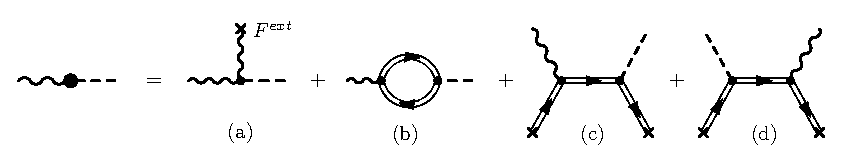
\includegraphics[width=15cm]{fig5_2.eps}}
\caption{ Диаграммы Фейнмана для эффективной вершины $\gamma a$ 
взаимодействия.}
\label{fig:vertexaxion}
\end{figure}



 В существующих аксионных моделях и в присутствии 
внешнего магнитного поля процесс  $i \to f+a$ 
можно описать эффективным лагранжианом вида~\cite{Raffelt:1996}:
%
\begin{eqnarray}
\label{eq:L1}
&&{\cal L}_{a\gamma}(x) = g_{a\gamma}\tilde F^{\mu \nu} [\partial_{\nu}A_{\mu}(x)] a(x) + 
\\
\nonumber
&& + \frac{g_{af}}{2m_f} 
[\bar \psi_f(x) \gamma^{\mu} \gamma_5 \psi_f(x)] \partial_{\mu} a(x) - 
%\\
%\nonumber
%&+&
 e_f[\bar \psi_f(x) \gamma^{\mu} \psi_f(x)]A_{\mu}(x) \, .
\end{eqnarray}
%
\noindent Напомним, что  $A_{\mu}$ -- четырехмерный потенциал квантованного электромагнитного
поля, $\tilde F^{\mu \nu}$ --  дуальный тензор внешнего поля,  $\psi_f(x)$  и $a(x)$ --  
квантованные фермионное и аксионное поля, 
  $g_{a\gamma} = \alpha \zeta/2\pi f_a$, $\zeta$ --  модельно зависимый 
параметр порядка единицы, 
$g_{af} = C_f m_f/f_a$ -- безразмерная Юкавская константа связи аксионов с 
фермионами с модельно зависимым фактором $C_f$, $e_f$ -- электрический заряд 
фермиона (для электрона $e_f = - e$). 

Исходя из лагранжиана~(\ref{eq:L1}) амплитуда процесса $i \to f + a$ может быть
представлена в следующем виде 
%
\begin{equation}
{\cal M}^a_{i \to f} 
 = - \frac{{\cal M}^{\gamma}_{if} {\cal M}_{\gamma \to a}}
{q'^2 -\varkappa^{(\varepsilon)}(q')}\, , 
\label{eq:M1if}                                                       
\end{equation}
%
\noindent где ${\cal M}^{\gamma}_{if}$ -- амплитуда процесса $i \to f + \gamma$  с 
излучением фотона в конечном состоянии,
%
\begin{equation}
{\cal M}_{\gamma \to a} 
 = i \bar g_{a\gamma} (\varepsilon \tilde F q') 
\label{eq:M2}                                                       
\end{equation}
%
\noindent --  амплитуда перехода фотон $\to$ аксион,  $q'^{\mu} = (\omega',{\bf k}')$ --   
четырехмерный импульс аксиона, $\varkappa^{(\varepsilon)}(q')$ -- собственное значение 
 поляризационного  оператора
фотона, которому соответствует вектор поляризации $\varepsilon_{\alpha}$. Эффективную  
константу аксион-фотонного взаимодействия, $\bar g_{a\gamma}$, можно 
представить в виде трех слагаемых: $\bar g_{a\gamma} = g_{a\gamma} + 
\Delta g^{B}_{a\gamma} + \Delta g^{pl}_{a\gamma}$.    
 Первое слагаемое соответствует взаимодействию 
аксиона с электромагнитным полем, обусловленному аномалией 
Адлера (диаграмма (a) на рис.~\ref{fig:vertexaxion}), второе обусловлено 
взаимодействием аксиона  с фотоном через электронную петлю 
(диаграмма (b) на рис.~\ref{fig:vertexaxion}), а третье --   
рассеянием вперед на электронах и позитронах плазмы (диаграммы (c) и (d) 
на рис.2). Подробный расчет $\Delta g^{B}_{a\gamma}$ и
$\Delta g^{pl}_{a\gamma}$ был сделан ранее в работах~\cite{Mikheev:1999} 
и~\cite{Mikheev:2006} соответственно. 
 Здесь мы отметим только, что для корректного вычисления величины $\Delta g^{B}_{a\gamma}$  
в ней необходимо 
 произвести вычитание, соответствующее аномалии Адлера~\cite{Mikheev:1999}. 
Этот факт, в 
частности, не был учтен в работе~\cite{Skobelev:2007}, что является одной из причин  
ошибочности полученных там результатов.

Далее представим $\varkappa^{(\varepsilon)}(q')$ в виде    
$\varkappa^{(\varepsilon)} = \Re - i\Im$, 
где $\Re = Re (\varkappa)$  реальная, а $\Im =  Im (\varkappa)$  мнимая части 
поляризационного оператора. Последняя обусловлена процессами поглощения и 
излучения фотонов в плазме и,
согласно~\cite{Weldon:1983}, следующим образом выражается через полную 
ширину рождения фотона, $\Gamma_{cr}$: 
%
\begin{eqnarray}
\label{eq:I1}                                                       
\Im = \omega' \left (e^{\omega'/T} - 1 \right ) \Gamma_{cr} ,  \quad 
%\\
%\nonumber 
\Gamma_{cr} = \sum_{i,f} \int  |{\cal M}^{\gamma}_{if}|^2 d\Phi_{if} ,
\end{eqnarray}
%
\noindent где $d\Phi_{if}$ --  элемент фазового объема состояний $i$ и $f$ для процесса 
$i \to f + \gamma$ с учетом соответствующих функций распределения,  
и сумма берется по всем возможным начальным и конечным состояниям. 

%С учетом вышесказанного, аксионная светимость за счет всевозможных реакций с участием 
%частиц плазмы может быть представлена  в виде 
%%
%\begin{equation}
%Q = \sum_{i,f} \int d\Phi_{if} \, d\Phi' \, \omega' 
%|{\cal M}^{\gamma}_{if}|^2 \, ,
%\label{eq:Qa0}                                                       
%\end{equation}
%%
%\noindent где $d\Phi' = \frac{d^3 k'}{(2\pi)^3 2 \omega'}$  фазовый объем аксиона. 
%
%С учетом~(\ref{eq:M1if}) и~(\ref{eq:I1}) $Q$ примет вид
%%
%\begin{equation}
%Q = \int  \frac{d\Phi' \, |{\cal M}_{\gamma \to a}|^2}{e^{\omega'/T} - 1} \, 
%\frac{\Im
%} 
%{(q'^2 -\Re)^2 + \Im^2} \, .
%\label{eq:Qa1}                                                       
%\end{equation}
%%
%
%Как видно из~(\ref{eq:Qa1}), наиболее существенный вклад в аксионную светимость будет
%давать область резонанса, т.е. окрестность точки пересечения дисперсионных кривых
%аксиона $q'^2 = m_a^2$ и фотона, $q'^2 = \Re$, так 
%что фотон становится реальным. В окрестности резонанса часть подынтегрального выражения
%в~(\ref{eq:Qa1}) можно интерполировать $\delta$-функцией:  
%%
%\begin{equation}
% \frac{\Im}
%{(q'^2 -\Re)^2 + \Im^2} \simeq \pi \, \delta(q'^2 -\Re) \, .
%\label{eq:Del1}
%\end{equation}
%%
%\noindent Воспользовавшись свойствами $\delta$-функции, перепишем~(\ref{eq:Del1})
% в виде  
%%
%\begin{equation}
% \frac{\Im}
%{(q'^2 -\Re)^2 + \Im^2} \simeq \pi \, 
%\int \frac{d^3 k}{2 \omega} Z_{\varepsilon} \delta^4 (q-q') \, ,
%\label{eq:Del2}
%\end{equation}
%%
%\noindent где  $Z_{\varepsilon}^{-1} = 1-\frac{\partial \Re}{\partial \omega^2}$ 
%соответствует перенормировке волновой функции фотона.
%
%
% С учетом~(\ref{eq:Del2}) cветимость~(\ref{eq:Qa1}) примет вид 
%%
%\begin{eqnarray}
%\label{eq:Qa2}
%Q &\simeq&  (2\pi)^4 \, 
%\int \frac{d^3 k}{2 \omega (2\pi)^3} \,\frac{\omega}{e^{\omega/T} - 1} \times
%\\
%\nonumber 
%&\times& \int \frac{d^3 k'}{2 \omega' (2\pi)^3}\, Z_{\varepsilon} 
%|{\cal M}_{\gamma \to a}|^2 \delta^4 (q-q') \, .
%\end{eqnarray}
%%
%\noindent Полученное выражение в точности соответствует формуле для аксионной светимости  
%в процессе $\gamma \to a$. Таким образом, аксионная светимость в 
%области резонанса за счет всевозможных  
%реакций с участием частиц среды 
%  однозначно выражается через светимость перехода фотон $\to$ 
%аксион.
%
%
%После интегрирования с $\delta$-функциями светимость приводится к виду
%%
%\begin{eqnarray}
%Q =  \frac{\bar g_{a\gamma}^2 (\beta)^2}{32 \pi^2 \alpha} \, 
%\int_{-1}^1 \frac{dx}{e^{\omega/T}-1} \, 
%\frac{Z_{\varepsilon} k 
%(\varepsilon \tilde \varphi q)^2}{\left |1-\frac{d\omega^2}{dk^2}\right |}\bigg |_{k=k^*}\, .
%\label{eq:Qa3}
%\end{eqnarray}
%%
%
%\noindent Здесь $x = \cos{\theta}$, $\theta$ --  угол 
%между направлением импульса фотона и магнитным полем, $k^* = k^*(\theta)$ --  
% корень уравнения $\omega^2 (\vec k) = m_a^2+k^2$. 
%% $\tilde \varphi_{\alpha \beta} = \tilde F_{\alpha \beta}/B$.
%
%
%Дальнейшее вычисление светимости будет существенно зависеть от характеристик плазмы, 
%определяющих, в конечном итоге, дисперсионные свойства фотонов. Здесь мы остановимся 
%на двух частных случаях.
%
%i) Слабо замагниченная плотная плазма,  $m_a^2 \ll \beta \ll T^2 , \mu^2$. В этом 
%случае в качестве $\varepsilon_\alpha$ будет выступать вектор поляризации продольного 
%плазмона
%%
%\begin{eqnarray}
%\varepsilon_\alpha = \sqrt{\frac{q^2}{(uq)^2-q^2}}\, 
%\left (u_\alpha - \frac{(uq)}{q^2}\, q_\alpha \right ) , 
%\end{eqnarray}
%%
%где $u_\alpha$ -- 4-скорость плазмы. Светимость~(\ref{eq:Qa3}) примет простой вид
%%
%\begin{eqnarray}
%Q =  \frac{\bar g_{a\gamma}^2 (\beta)^2}{48 \pi^2 \alpha} \, 
% \frac{(k^*)^3}{e^{k^*/T}-1} \, 
%\label{eq:Qa4}
%\end{eqnarray}
%%
%
%\noindent 
%в полном согласии с результатом работы~\cite{MRV:1998}. Отметим, что в данном пределе 
% величина $k^*$ не зависит от $\theta$, а определяется только параметрами плазмы.
%
%
%ii) Сильно замагниченная нерелятивистская холодная плазма  $\beta \gg m^2$, $\mu^2 \gg T^2$. Здесь %\newline   
%$\varepsilon_\alpha = 
%(q \tilde \varphi)_\alpha/\sqrt{q^2_{\mprl}}$, 
%$\Re \simeq (q \tilde \varphi \tilde \varphi q) \left (\frac{\omega_p^2(1+\xi)}{\omega^2} -
%\xi \right )$, и плазменная частота $\omega_p$   
%следующим образом связана с концентрацией электронов:  $\omega^2_p = 4\pi \alpha n/m$; $\xi = (\alpha/3\pi)(B/B_e)$. 
%Кроме того, в рассматриваемом пределе 
%$\bar g_{a\gamma} \simeq g_{a\gamma}$. Однако,  
%в отличие от случая слабо замагниченной плазмы, светимость до конца интегрируется
%лишь в некоторых частных случаях:
%
%\begin{itemize} 
%
%\item масса аксиона --  наименьший параметр задачи, т.е. 
%$\omega_p, \,T \gg m_a$ (например, рождение легких, с массой меньшей, чем 
%$10^{-5}$\,эВ, аксионов в магнитосфере
%магнитара).  % (см. формулу~(\ref{eq:n1}))). 
%В этом случае 
%$k^* \simeq \omega_p \sqrt{1+1/\xi}$ и светимость~(\ref{eq:Qa3}) примет вид
%%
%\begin{eqnarray}
%\label{eq:Qa5a}
%Q &\simeq&  \frac{g_{a\gamma}^2 (\beta)^2}{16 \pi^2 \alpha} \,
%\omega_p^3 \frac{(1+\xi)^{3/2}}{\xi^{5/2}}\times
%\\
%\nonumber 
%&\times& \left (\exp{\left [\frac{\omega_p}{T} 
%\sqrt{1+\frac{1}{\xi}}\, \right ]}-1 \right )^{-1} \, .
%\end{eqnarray}
%%
%
%
%\item $\omega_p \gg T \sim m_a$. Анализ показывает, что в этом 
%случае интеграл в~(\ref{eq:Qa3}) набирает
%свою величину в области $x\simeq 1$, и, следовательно, $k^* \simeq \omega_p $.
%  Тогда светимость примет вид
%%
%\begin{eqnarray}
%\label{eq:Qa5b}
%Q &\simeq&  \frac{g_{a\gamma}^2 (\beta)^2}{16 \pi^2 \alpha} \, T m_a^2  \, 
%e^{-\omega_p/T} \, .
%\end{eqnarray}
%%
%
%\end{itemize}

Представляет самостоятельный интерес оценка количества аксионов,
рождаемых в магнитосфере магнитара в единице объема за единицу времени с 
помощью рассмотренного выше резонансного
механизма, поскольку аксион является одним из основных кандидатов в составляющие
холодной темной материи. Аналогично~(\ref{eq:Qa3}), (\ref{eq:Qa5a}) 
и~(\ref{eq:Qa5b}) получаем: 
%
\begin{eqnarray}
\frac{dN}{dt dV} =  \frac{g_{a\gamma}^2 (\beta)^2}{32 \pi^2 \alpha} \, 
\int_{-1}^1 \frac{dx}{e^{\omega/T}-1} \, 
%\frac{k}{\omega} \, 
\frac{k Z_{\varepsilon} 
(\varepsilon \tilde \varphi q)^2}{\omega 
\left |1-\frac{d\omega^2}{dk^2}\right |}\bigg |_{k=k^*}\, ,
\label{eq:Na0}
\end{eqnarray}
%

%
\begin{eqnarray}
\label{eq:Na1}
\frac{dN}{dt dV} &\simeq&  \frac{g_{a\gamma}^2 (\beta)^2}{16 \pi^2 \alpha} \,
\omega_p^2 \frac{1+\xi}{\xi^{2}}\times
\\
\nonumber 
&\times& \left (\exp{\left [\frac{\omega_p}{T} 
\sqrt{1+\frac{1}{\xi}}\, \right ]}-1 \right )^{-1} \, , \quad \omega_p,\, T \gg m_a,
\end{eqnarray}
%

%
\begin{eqnarray}
\label{eq:Na2}
\frac{dN}{dt dV} &\simeq&  \frac{g_{a\gamma}^2 (\beta)^2}{16 \pi^2 \alpha} \,
\frac{T m_a^2}{\omega_p}  \, e^{-\omega_p/T} \, , \quad \omega_p \gg T \sim m_a.
\end{eqnarray}
%



В частности, для числа аксионов, рождаемых реликтовым излучением 
($T \sim m_a \sim 10^{-3}$\,эВ), при  
 минимальной  концентрации плазмы ($\sim 10^{15}$\,см$^{-3}$), при которой все еще 
 реализуется  резонансный механизм $(\omega_p \gtrsim  m_a)$ и величине магнитного поля 
 $B=100B_e$, получаем из~(\ref{eq:Na0})  
следующую максимальную оценку $dN/(dV dt)\sim 10^{10}$ штук в см$^{-3}$ за секунду. 
 Таким образом, в объеме магнитосферы магнитара 
 ($\sim 10^{19}$\,см$^3$), заполненной сильным магнитным полем,  рождается за секунду 
 $10^{29}$ аксионов. Оценивая в самом оптимистичном варианте 
 число магнитаров в Галактике $\sim 10^6$, получаем, 
 что за $\sim 10^9$ лет они произведут $\sim 10^{51}$ аксионов, и, следовательно, 
 концентрация  аксионов в Галактике должна быть  $n_a \sim 10^{-21}$\,см$^{-3}$. Это число
 можно сравнить, например, с концентрацией барионов $n_b \sim 10^{-7}$\,см$^{-3}$ $\gg n_a$.  
Следовательно, данный механизм не дает возможность генерации аксионной составляющей <<холодной скрытой массы>>. 
% Следовательно, утверждение автора~\cite{Skobelev:2007} о том, что <<окрестности 
% магнитных нейтронных 
% звезд с полями $B \gg B_e$ могут являться мощными генераторами по преобразованию 
% реликтового излучения в аксионную составляющую холодной скрытой массы>> не является 
% верным.
 
 